\documentclass[xcolor=table,ignorenonframetext,12pt,handout]{beamer} %,handout
%\documentclass[xcolor=table,handout,12pt]{beamer}
\usepackage[frenchb]{babel}
\usepackage[latin1]{inputenc}
\usepackage{amsmath,amssymb}
\usepackage{graphicx}
\usepackage{pgfarrows,pgfnodes}
\usepackage{url}
\usepackage{textcomp}
\usepackage[vcentermath]{youngtab}
\usepackage{epstopdf}
\usepackage{hhline}
\usepackage{xmpmulti}
\usepackage{subfigure}
\usepackage{tikz}
\usepackage{multirow}

\mode<article> {
  \usepackage{fullpage}
  \usepackage{pgf}
  \usepackage{hyperref}
}
\newcommand{\til}{TaxIPP-Life}

\mode<presentation>

%\usetheme[left]{Goettingen}
%\setbeamertemplate{background canvas}{\includegraphics[width=\paperwidth]{ippheader.pdf}}
\setbeamertemplate{background canvas}{\hspace{10.1cm}\includegraphics
    [width=0.2\paperwidth]{logo_ipp.pdf}}
\definecolor{ippdark}{RGB}{0,93,116}
\definecolor{ipplight}{RGB}{0,142,156}
\useinnertheme[shadow=true]{rounded}
\setbeamertemplate{items}[circle]
\setbeamercolor{title}{bg=ipplight, fg=black}
\setbeamercolor{structure}{fg=ipplight}
%\setbeamertemplate{sidebar canvas left}{} % pour supprimer le fond de couleur de la barre lat�rale	
\setbeamertemplate{sidebar canvas left}[vertical shading][top=structure.fg!20,bottom=structure.fg!15]
\setbeamertemplate{caption}[numbered]
\setlength{\leftmargini}{12pt}
\setbeamerfont{framesubtitle}{size=\large}

%\usepackage[latin1]{inputenc}
%\usepackage[english]{babel}

\newenvironment{checklist}[1]{\begin{list}{$\surd$}{}#1}{\end{list}}%
\newcommand{\graphique}[2][1]{\begin{minipage}{\linewidth}\begin{center}\includegraphics[width=#1\linewidth,clip]{#2}\end{center}\end{minipage}}%
\newcommand{\os}[2]{\onslide+<#1->{#2}}%

\newcommand{\m}[2]{\multicolumn{#1}{c}{#2}}%
\newcommand{\ml}[2]{\multicolumn{#1}{l}{#2}}%
\newcommand{\tth}{\textsuperscript{th}}%
\newcommand{\nde}{\textsuperscript{nde}}
\newcommand{\hligne}{\begin{tikzpicture}[remember picture,overlay]\node[shift={(-10.5 cm,-1.2cm)}]at(current page.north east){\begin{tikzpicture}{\draw[line width=0.2mm,color=ipplight,overlay](0,0)--(8,0);}\end{tikzpicture}};\end{tikzpicture}\vspace{-0.8cm}}
\newcommand{\hlignee}{\begin{tikzpicture}[remember picture,overlay]\node[shift={(-10.5 cm,-1.2cm)}]at(current page.north east){\begin{tikzpicture}{\draw[line width=0.2mm,color=ipplight,overlay](0,0)--(8,0);}\end{tikzpicture}};\end{tikzpicture}}

% MTABLE: macro for tables %
\newenvironment{mfigure}[4][1]{\def\TMP{#3}\newdimen\TMPsize\settowidth{\TMPsize}{\TMP}
\begin{figure}\caption{#2}\begin{center}\begin{tiny}
\begin{minipage}{#1\textwidth}\resizebox{\textwidth}{!}{#3}\end{minipage}
\if!#4!\empty \else \\
\resizebox{#1\textwidth}{!}{\begin{minipage}{\TMPsize}\begin{tiny}\smallskip\par
#4 \end{tiny}\end{minipage}} \fi}
{\end{tiny}\end{center}\end{figure}}

\makeatletter
\def\TAXIPP{TAX\kern-.05em\lower-.19ex\hbox{${\color{BlueGreen} \scalebox{1.4}{\underarc[1]{\overarc[1]{\textcolor{black}{\scalebox{0.7}{ipp}}}}}}\hspace{0.5ex}$}\@}
\makeatother

\title{TAXIPP-LIFE microsimulation model\\ A life-cycle point of view}
\author{Alexis Eidelman}
\institute{\emph{Institut des politiques publiques}}
\subject{Redistribution ; microsimulation ; Life-Cycle}

\date{IFS informal seminar \\London -- 20th of June 2013}

\begin{document}

\frame{\maketitle}

\section*{Introduction}
\begin{frame}
\frametitle{Introduction}
\framesubtitle{\vspace{0.3cm}General overview of \til}
\begin{itemize}
	\item Dynamic microsimulation model developed by \textit{Institut des politiques publiques} (IPP)
	\item Ageing and legislation \pause
	\item Reforms
	\item \textbf{Work in progress} \pause
%\item \textbf{Importance de la perspective de cycle de vie}
%    \begin{enumerate}
%      \item Pour l'�tude des niveaux de vie et des in�galit�s
%\item Pour l'�tude de la redistribution op�r�e par les syst�mes fiscalo-sociaux
%    \end{enumerate} \pause
%    \item \textbf{Structure du mod�le}
%    \begin{itemize}
%    \item Donn�es r�trospectives r�ellement observ�es
%    \item Simulation des trajectoires futures
%    \end{itemize}
\end{itemize}
\end{frame}

\begin{frame}
\frametitle{Roadmap}
  \tableofcontents[hideothersubsections] 
\end{frame} 

\section{Why to be interested in Life-Cycle ?}
\subsection{Inequalities}
\begin{frame}
\frametitle{Roadmap}
  \tableofcontents[currentsection, hideothersubsections] 
\end{frame} 

\begin{frame}
\frametitle{Why to be interested in Life-Cycle ?}
\framesubtitle{\vspace{0.3cm} Evaluation inequalities} \pause
\begin{itemize}
	\item Annual income doesn't measure utility (or living standard)
		\begin{enumerate}
		\item Income chocks (plus value, unemployment, child care, bad harvest)
		\item Different period of life (studies, retirement)
		\item Wealth (and inheritance) can't be ignored
		\end{enumerate}
	On administrative (Swedish) data, it was measured that 40\% \ of Gini-inequalities are intra-personal. 
\end{itemize}
\end{frame}

\subsection{Redistribution}

\begin{frame}
\frametitle{Why to be interested in Life-Cycle ?}
\begin{enumerate}
\item Who is rich and who is poor ?
\item Who does give money to whom through redistibution ?
\end{enumerate}
\end{frame}

\begin{frame}
\frametitle{Why to be interested in Life-Cycle ?}
\framesubtitle{\vspace{0.3cm} Redistribution} 
\begin{itemize}
\item \textbf{Two extreme cases}
	\begin{itemize}
	\item People with same income during their whole life \\
	$\Rightarrow$ Redistribution between people \pause
	\item Same individuals with variation in income but born at different times \\
	$\Rightarrow$ Redistribution "within" people only \\
	(Useless if credit and assurance market are perfect)
	\end{itemize}
\end{itemize} \pause
 \footnotesize
\begin{table}	
\caption{Share of within redistribution in whole redistribution}
 \begin{tabular}{|c|c|c|}
\hline
Pettersson and Pettersson (2007) &      Sweden &  18-32 \% \\
\hline
Hussenius and Selen (1994) &      Sweden &  24-32 \% \\
\hline
Falkingham and Harding (1996) &  Australia &  48-63 \% \\
\hline
Falkingham and Harding (1996) & United-Kingdom &  29-38 \% \\
\hline
O'Donoghue &    Ireland &     45 \% \\
\hline
O'Donoghue &     Italy &     24 \% \\
\hline
\end{tabular}
\end{table}
\end{frame}

\begin{frame}
\frametitle{Why to be interested in Life-Cycle ?}
\framesubtitle{\vspace{0.3cm} Redistribution} 
\begin{itemize}
	\item People may contribute and benefit from the tax and benefit system at different periods. \\
	
	 \ House benefit for students (or others state services) \pause
	\item Assurance issue
		\begin{enumerate}
		\item unemployment benefit, health care, pension system
		\item Forced consumption? \\	
		\ 	$\longrightarrow$ no redistribution
		\item But a contribution may not equal risk expectancy \\
		\	$\longrightarrow$ redistribution
	\end{enumerate}
\end{itemize}
\end{frame} 

\subsection{Particular fields}
\begin{frame}
\frametitle{Why to be interested in Life-Cycle ?}
\framesubtitle{\vspace{0.3cm} Particular fields} 
\begin{itemize}
	\item A life-cycle perspective is unavoidable when careers is a major point   \\
	\	$\longrightarrow$ pension, educational choice
	\item Can add very interesting point in particular when demography is at stake. \\
	\	$\longrightarrow$ Female labour, health (end of life)	
\end{itemize} \pause
The aim of \til \ is to be as general as possible and not focused on a specific topic.

\end{frame} 

\subsection{Getting more general}

\begin{frame}
\frametitle{Why to be interested in Life-Cycle ?}
\framesubtitle{\vspace{0.3cm}Getting more general-1} 
\begin{itemize}
	\item Enable to study reform at upper level
	 \begin{itemize}
		\item Impact of pension reform on age departure and educational choice
		\item Impact of ageing population on retirement home supply and on house pricing (and housing benefits)
	 \end{itemize}
	\item Objective to have a complete economic informations on people \pause
	\item Requires an organisation and some organisation	
\end{itemize} 
\end{frame} 

\begin{frame}
\frametitle{Why to be interested in Life-Cycle ?}
\framesubtitle{\vspace{0.3cm}Getting more general-2} 
\begin{itemize}
	\item Evaluate a reform not in a cross section framework
	 \begin{itemize}
		\item Already done for pensions for example
		\item But what about tax income on pension ? Or family benefit.
		\item Number of impacted people ? 
	 \end{itemize}
	\item Interest in hypothetical past reforms.
\end{itemize} 
\end{frame} 


\section{Some issues for a dynamic microsimulation model}

\begin{frame}
\frametitle{Roadmap}
  \tableofcontents[currentsection, hideothersubsections] 
\end{frame} 


\subsection{Data}
\begin{frame}
\frametitle{Data}
\begin{itemize}
\item \textbf{Issue: } To know people's past and on careers (administrative data) and on marital status (survey data).
\item \textbf{How \til \ deals with:}  \pause
	\begin{itemize}
	\item French wealth survey
	\item Administrative data (pension)
	\item Statistical matching 
	\begin{itemize}
	\item  Exact matching on sex, age, kind of work
	\item  Distance for income in 2009
	\item  Optimal matching for career (replacement, insertion, deletion cost)\\
		$\longrightarrow$ closest neighbour
	\end{itemize}	\pause
	\item Survey closure
	\end{itemize} \pause
\item \textbf{How to get better: }
	\begin{itemize}
	\item Other surveys (Health survey)
	\item Joint selection for parents
	\end{itemize} \pause 
\item \textbf{Issue: } To know people's future	
\end{itemize}
\end{frame}

\subsection{Survey weight}
\begin{frame}
\frametitle{Survey weight}
\begin{itemize}
\item \textbf{Issue: } Links between people change in a dynamic simulation. How link two individuals with different weight. \pause
\item \textbf{How \til \ deals with:} 
	\begin{itemize}
	  \item Work with uniform weight
	  \item Replication according to weight
	  \item Increase variability \pause
	  \item No real other option
	\end{itemize}
\item \textbf{How to get better: } \pause
	\begin{itemize} \pause
	\item Smallest weight in wealth survey is 6 ! \\
	$\rightarrow$ 11 millions individuals
	\item  200 is our constant weight  \\
	$\rightarrow$ 300 000 individuals \\
	\item Go further in survey size
	\end{itemize}
\end{itemize}
\end{frame}

\subsection{Time scale}
\begin{frame}
\frametitle{Time scale}
\begin{itemize}
\item \textbf{Issue: } A trade-off between precision and calculus time.
\item \textbf{How \til \ deals with:}  \pause
	\begin{itemize}
	\item So far : annual scale
	\item Possibility to run some process on a longer basis
	\end{itemize} 
\item \textbf{How to get better: }
	\begin{itemize}
	\item Month scale
	\item ...or at least trim scale
	\item Simulate durations more than transitions
	\end{itemize}
\end{itemize}
\end{frame}

\subsection{Marriage}
\begin{frame}
\frametitle{Marriage}
\begin{itemize}
\item \textbf{Issue: } To marry people verifying a given joint distribution of characteristics. A trade-off between optimality and computational intensity. \pause
\item \textbf{How \til \ deals with:}  
	\begin{itemize}
	\item Not a marriage market
	\item Distance between people
	\item Minimisation Algorithm
	\end{itemize} \pause
\item \textbf{How to get better: } \pause
	\begin{itemize}
	\item Improve minimisation algorithm (Hungarian method)
	\item Randomly select some potential match and run the optimisation on that subset
	\end{itemize}
\end{itemize}
\end{frame}

\subsection{Alignment}
\begin{frame}
\frametitle{Alignment}
\begin{itemize}
\item \textbf{Issue: } High volatility for number of events simulated by a binary model. \pause
\item \textbf{How \til \ deals with:}  \pause
	\begin{itemize}
	\item Use an already implemented technique of Liam2 (see Li and O'Donoghue 2012)
	\end{itemize} \pause
\item \textbf{How to get better: } 
	\begin{itemize}
	\item Try other techniques.
	\end{itemize}
\end{itemize}
\end{frame}


\subsection{Individualisation}
\begin{frame}
\frametitle{Individualisation}
\begin{itemize}
\item \textbf{Issue: } In a life-cycle point of view, the lonely pertinent entitiy is the individual. But living standards, benefits and sometimes taxes are calculated at a bigger level (household, couple, family). How individualize? \pause
\item \textbf{How \til \ deals with:}  
	\begin{itemize}
	\item Income tax split between spouse.
	\item but tax reduction related to children which is split between children.
	\item Family benefit split between children.
	\item Other benefits split between all household members.
	\end{itemize} \pause
\item \textbf{How to get better: }
	\begin{itemize}
	\item Be more precise but...
	\item ...is not the Shapley Value the lonely solution?
	\end{itemize}
\end{itemize}
\end{frame}




\subsection{Programming language}
\begin{frame}

  \frametitle{Programming language}
  \framesubtitle{\vspace{0.3cm}Organisation}
  \begin{itemize}
  \item \textbf{Langages}
    \begin{itemize}
    \item Initial work on data in R
    \item Motor in Python
    \item User-friendly Text Interface (YAML)
    \end{itemize}
     \item \textbf{Why Python} ?\pause
    \begin{itemize}
    	\item Clear
    	\item Possibility to look at a particular point.
		\item Way much faster than statistical language.
    \end{itemize}
	\item A choice made by Liam2 et OpenFisca.
	\item Simulation on 30 000 individuals : \  6 s/period
	\item Simulation on 300 000 individuals : 70 s/period
  \end{itemize}
\end{frame}

\begin{frame}[plain,t]
\frametitle{Athlete struggling with a python}
\begin{center}
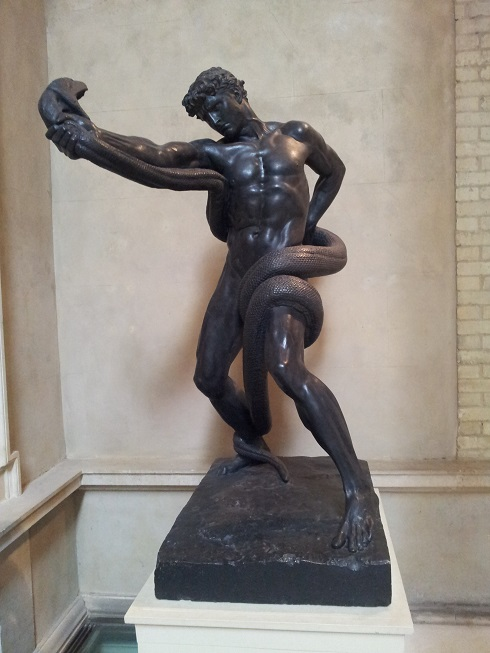
\includegraphics[0.8]{struggling_with_Python.jpg}
\end{center}
\end{frame}

\section{How \til \ simulate}
\begin{frame}
\frametitle{Roadmap}
  \tableofcontents[currentsection, hideothersubsections] 
\end{frame} 


\subsection{Entities and links}
\begin{frame}
\frametitle{Entities and links}
\framesubtitle{\vspace{0.3cm}Organisation}
\begin{itemize}
\item \textbf{Entities} \\
4 entities (one is not vital)
	\begin{itemize}
	\item Individuals
	\item House
	\item Income Declaration
	\item Companies 
	\end{itemize} \pause
\item + a \textbf{register} \pause
\item \textbf{Links}
	\begin{itemize}
	\item Links between persons : spouse and parents.
	\item Links from persons to their entities
	\item Links from entities to their owners
	\end{itemize} 
\end{itemize}
\end{frame}


\subsection{Simulation Processes}
\subsubsection{Demography}
\begin{frame}
\frametitle{Simulation Processes}
\framesubtitle{Demography - 1}
\begin{itemize}
\item Birth \\
\begin{itemize}
\item Women in a couple, alignment on birth per age.
\item No (direct) correlation with education, nor previous children
\end{itemize}
\item Independence
\begin{itemize}
\item At a deterministic age given education level
\item No other moving
\end{itemize}
\end{itemize}
\end{frame}

\begin{frame}
\frametitle{Simulation Processes}
\framesubtitle{Demography - 2}
\begin{itemize}
\item Marriage \\
	\begin{itemize}
	\item Equations taken from Destinie microsimulation model
	\item Probability to look for a spouse depends on age, leaving eduction age, time since previous union and number of child
	\item Matching depends only on age and education
	\item Children follow their parents (in household and income declaration)
	\end{itemize}
\item Divorce
	\begin{itemize}
	\item Depends on couple's duration, number of children and age difference.
	\item Children follow randomly mother or father.
	\end{itemize}
\end{itemize}
\end{frame}


\begin{frame}
\frametitle{Simulation Processes}
\framesubtitle{Demography - 3}
\begin{itemize}
\item Death \\
	\begin{itemize}
	\item Alignment according to age and sex
	\item Income and education are not taken into account
	\item \textbf{Inheritance} (including second order inheritance)
	\item Tax on inheritance 
	\item No car accident
	\end{itemize}
\end{itemize}
\end{frame}

\subsubsection{Job market}
\begin{frame}
\frametitle{Simulation Processes}
\framesubtitle{Status}
\begin{itemize}
\item Education
	\begin{itemize}
	\item Depends only on parental educational background.
	\item Classes just depends on age
	\end{itemize}
\item Job market
	\begin{itemize}
	\item Simple equations and rough alignment
	\item No part-time job.
	\end{itemize}
\item Retirement
	\begin{itemize}
	\item Systematic with age
	\item PENSIPP could do the job
	\end{itemize}
\end{itemize}
\end{frame}

\begin{frame}
\frametitle{Simulation Processes}
\framesubtitle{Income}
\begin{itemize}
\item In work
	\begin{itemize}
		\item Salary on a Mincer equation...
		\item ... and an observed or simulated personal productivity
	\end{itemize}
\item Pension
	\begin{itemize}
		\item Pension depends only on last salary
		\item PENSIPP could do the job
	\end{itemize}
\item Unemployment benefit
	\begin{itemize}
	\item Code written
	\item but not very relevant with year time scale
	\end{itemize}
\end{itemize}
\end{frame}


\subsubsection{Consumption and savings}
\begin{frame}
\frametitle{Simulation Processes}
\framesubtitle{Consumption and savings}
\begin{itemize}
\item Need new estimation
	\begin{itemize}
	\item taking life-cycle as a parameter
	\item individualisation 
	\end{itemize}
\end{itemize}
\end{frame}

%\subsubsection{D�veloppements futurs}
%\begin{frame}
%  \hligne
%  \frametitle{III. Les �tapes de la simulation - activit� }
%  \begin{itemize}
%	\item Il y a encore beaucoup de champs qui pourrait �tre travaill�s
%  	\begin{itemize}
%	\item Sant� et d�pendance
%	\item Mode de garde
%	\item Choix d'�ducation
%  	\end{itemize}
%  \end{itemize}
%\end{frame}


\section{Becoming of \til}
\begin{frame}
\frametitle{Roadmap}
\tableofcontents[currentsection, hideothersubsections] 
\end{frame} 

\begin{frame}
\frametitle{Becoming of \til}
\framesubtitle{\vspace{0.3cm} First stage: a suspended time}
\begin{itemize}
\item Legislation and population of 2009
\begin{itemize}
\item No growth ( nor trend)
\item Revaluation of past income
\item Only 2009 legislation is applied
\end{itemize}
\item Not deal with past union and divorce (in progress).
\end{itemize}
\end{frame}

\begin{frame}
\frametitle{Becoming of \til}
\framesubtitle{\vspace{0.3cm} Response}
\begin{itemize}
\item Reform can be implemented after the simulation \pause
\item But also after each period \\
	$\rightarrow$ Response \pause
\item A midterm goal is to have a decision model
\end{itemize}
\end{frame}

\begin{frame}
\frametitle{Becoming of \til}
\framesubtitle{\vspace{0.3cm} Development}
\begin{itemize}
\item OpenFisca can deal with other countries \\ \pause
	$\rightarrow$ Is French legislation different or are French different? \pause
\item Becoming of \til \ linked to becoming of IPP \pause
\item Becoming of \til \ \textbf{not} \ linked with mine, I hope.
\item To be continued...
\end{itemize}
\end{frame}

\frame{\maketitle}

\end{document}
